% Ta dokument je bil ustvarjen na osnovi predloge za poročila o domačih
% nalogah, katere nosilec je Blaž Zupan in je dostopna na spletni učilnici
% predmeta UOZP.

\documentclass[a4paper,11pt]{article}
\usepackage{a4wide}
\usepackage{fullpage}
\usepackage[utf8x]{inputenc}
\usepackage[slovene]{babel}
\selectlanguage{slovene}
\usepackage[toc,page]{appendix}
\usepackage[pdftex]{graphicx} % za slike
\usepackage{setspace}
\usepackage{color}
\definecolor{light-gray}{gray}{0.95}
\usepackage{listings} % za vključevanje kode
\usepackage{hyperref}
\usepackage{titlesec}
\usepackage{amsmath}
\usepackage{amsthm}

\renewcommand{\baselinestretch}{1.1} % za boljšo berljivost večji razmak
\renewcommand{\appendixpagename}{\normalfont\Large\bfseries{Priloge}}

\lstset{ % nastavitve za izpis kode
language=Python,
basicstyle=\footnotesize,
basicstyle=\ttfamily\footnotesize\setstretch{1},
backgroundcolor=\color{light-gray},
}

\title{\textbf{Strojno učenje za boljšo povečavo slik}}
\author{Blaž Rojc}
\date{\today}

\begin{document}

\maketitle

% 1
\section{Uvod}

Današnja fotografska oprema, od profesionalnih fotoaparatov do pametnih telefonov, je zmožna zajemati slike v visokih ločljivostih.
Ker pogosto polna ločljivost slike ni potrebna, se večina slik pred shranjevanjem ali pošiljanjem zmanjša.

To samo po sebi ne bi bil problem, če bi se za spreminjanje velikosti uporabljali algoritmi, ki bi skušali čim bolj ohraniti kvaliteto slike.
Ampak zaradi minimizacije stroškov procesiranja in shranjevanja veliko aplikacij uporablja bilinearno interpolacijo\footnote{\url{
	https://en.wikipedia.org/wiki/Bilinear\_interpolation}}, ki zelo hitro spremeni velikost slike na račun kvalitete.

S ciljem boljše povečave slik sem ustvaril konvolucijsko nevronsko mrežo, ki vzame bilinearno interpolirano, v vsako dimenzijo štirikrat povečano sliko
	in vrne izboljšano verzijo z manj artifakti povečave.
V tem besedilu bom predstavil delovanje nevronske mreže, njeno obliko, programsko okolje, ki sem ga uporabil, in množico slik, uporabljeno
	pri učenju in preizkušanju mreže.

Pri načrtovanju mreže sem se usmerjal po raziskavah s podobnim namenom.\cite{intel1, intel2, intel3}
V večini primerov je šlo za večslojne nevronske mreže, jaz sem se pa omejil na en sloj s konvolucijo.

Rezultati so sprejemljivi, mreža je zmožna očitno izboljšati kvaliteto slike v primerjavi z bilinearno interpolacijo samo.

% 2
\section{Definicije}

%V tem besedilu so večkrat uporabljeni izrazi \emph{konvolucija}, \emph{aktivacijska funkcija} in \emph{konvolucijska nevronska mreža}.
%Definirajmo jih.

\subsection{Konvolucija}

\emph{Konvolucija} \cite{torch_conv2d} je računska operacija, podana s formulo

\begin{equation*}
\text{izhod}(C_{izhod_j}) =
	\text{odmik}(C_{izhod_j}) + \sum_{\substack{C_{vhod_i} \\ \in C_{vhod}}} \text{utež}(C_{izhod_j}, C_{vhod_i}) \star \text{vhod}(C_{vhod_i}) \text{,}
\end{equation*}

kjer sta $C_{izhod_j}$ in $C_{vhod_i}$ barvna kanala slike, $C_{vhod} = C_{izhod} = (\text{rdeč}, \text{zelen}, \text{moder})$,
	oznaka $\star$ pa označuje \emph{diskretno korelacijo}, podano s formulo

\begin{equation*}
(f\star g) (n) = \sum_{m = - \infty}^{\infty} \overline{f(m)} \cdot g(m + n) \text{.}
\end{equation*}

Oznaka $\overline{f}$ nakazuje, da gre za kompleksno konjugiranko $f$, ampak ker so vsi vhodi, uteži in odmiki realna števila,
	uporabljamo pa le operaciji seštevanja in množenja, velja $\overline{f} = f$ in enačbo lahko zapišemo v obliki

\begin{equation*}
(f\star g) (n) = \sum_{m = - \infty}^{\infty} f(m) \cdot g(m + n) \text{.}
\end{equation*}

Vemo, da ima funkcija uteži končno definicijsko območje, zato se omejimo le na $k$ členov:

\begin{equation*}
(f\star g) (n) = \sum_{m = 0}^{k - 1} f(m) \cdot g(m + n)
\end{equation*}

Število k imenujemo \emph{jedro konvolucije}.

Slike so dvodimenzionalni objekti, v računalniku predstavljeni kot trojica dvodimenzionalnih matrik - vsaka predstavlja intenzivnosti
	enega izmed treh barvnih kanalov.\footnote{\url{https://en.wikipedia.org/wiki/Raster\_graphics}}
Torej moramo pojem konvolucije razširiti na dve dimenziji:

\begin{equation*}
(f\star g) (x, y) = \sum_{m, n = 0}^{k - 1} f(m, n) \cdot g(x + m, y + n)
\end{equation*}

Vstavimo sedaj to formulo v definicijo konvolucije in računajmo za točko $(x, y)$:

\begin{multline*}
\text{izhod}(C_{izhod_j}, x, y) = \\
	\text{odmik}(C_{izhod_j}, x, y) + \sum_{\substack{C_{vhod_i} \\ \in C_{vhod}}} \sum_{m, n = 0}^{k - 1}
	\text{utež}(C_{izhod_j}, C_{vhod_i}, m, n) \cdot \text{vhod}(C_{vhod_i}, x + m, y + n)
\end{multline*}

Opazimo: `vhod', `izhod' in `odmik' so trodimenzionalne podatkovne strukture, `utež' pa kar štiridimenzionalna.
Take strukture imenujemo \emph{tenzorji}.

\subsection{Aktivacijska funkcija}

Izraz \emph{aktivacijska funkcija} označuje funkcijo, ki izhodno vrednost sloja mreže preslika v vrednost v želenem območju.\cite{activation_func_1}
V globokih nevronskih mrežah se aktivacijske funkcije uporabljajo za vnos nelinearnosti,
	ki omogoča smiselno komponiranje operacij.\cite{activation_func_2}

Nekaj primerov aktivacijskih funkcij predstavljajo usmerjena linearna enota (ReLU):
\begin{equation*} 
f(x) = \begin{cases}
	0 & \text{za } x < 0 \\
	x & \text{za } x \ge 0,
\end{cases}
\end{equation*}
sigmoid:
\begin{equation*} 
f(x) = \frac{1}{1 + e^{-x}},
\end{equation*}
in binarna stopnica:
\begin{equation*} 
f(x) = \begin{cases}
	0 & \text{za } x < 0 \\
	1 & \text{za } x \ge 0.
\end{cases}
\end{equation*}

\subsection{Nevronska mreža}

\begin{figure}[htbp]
\begin{center}
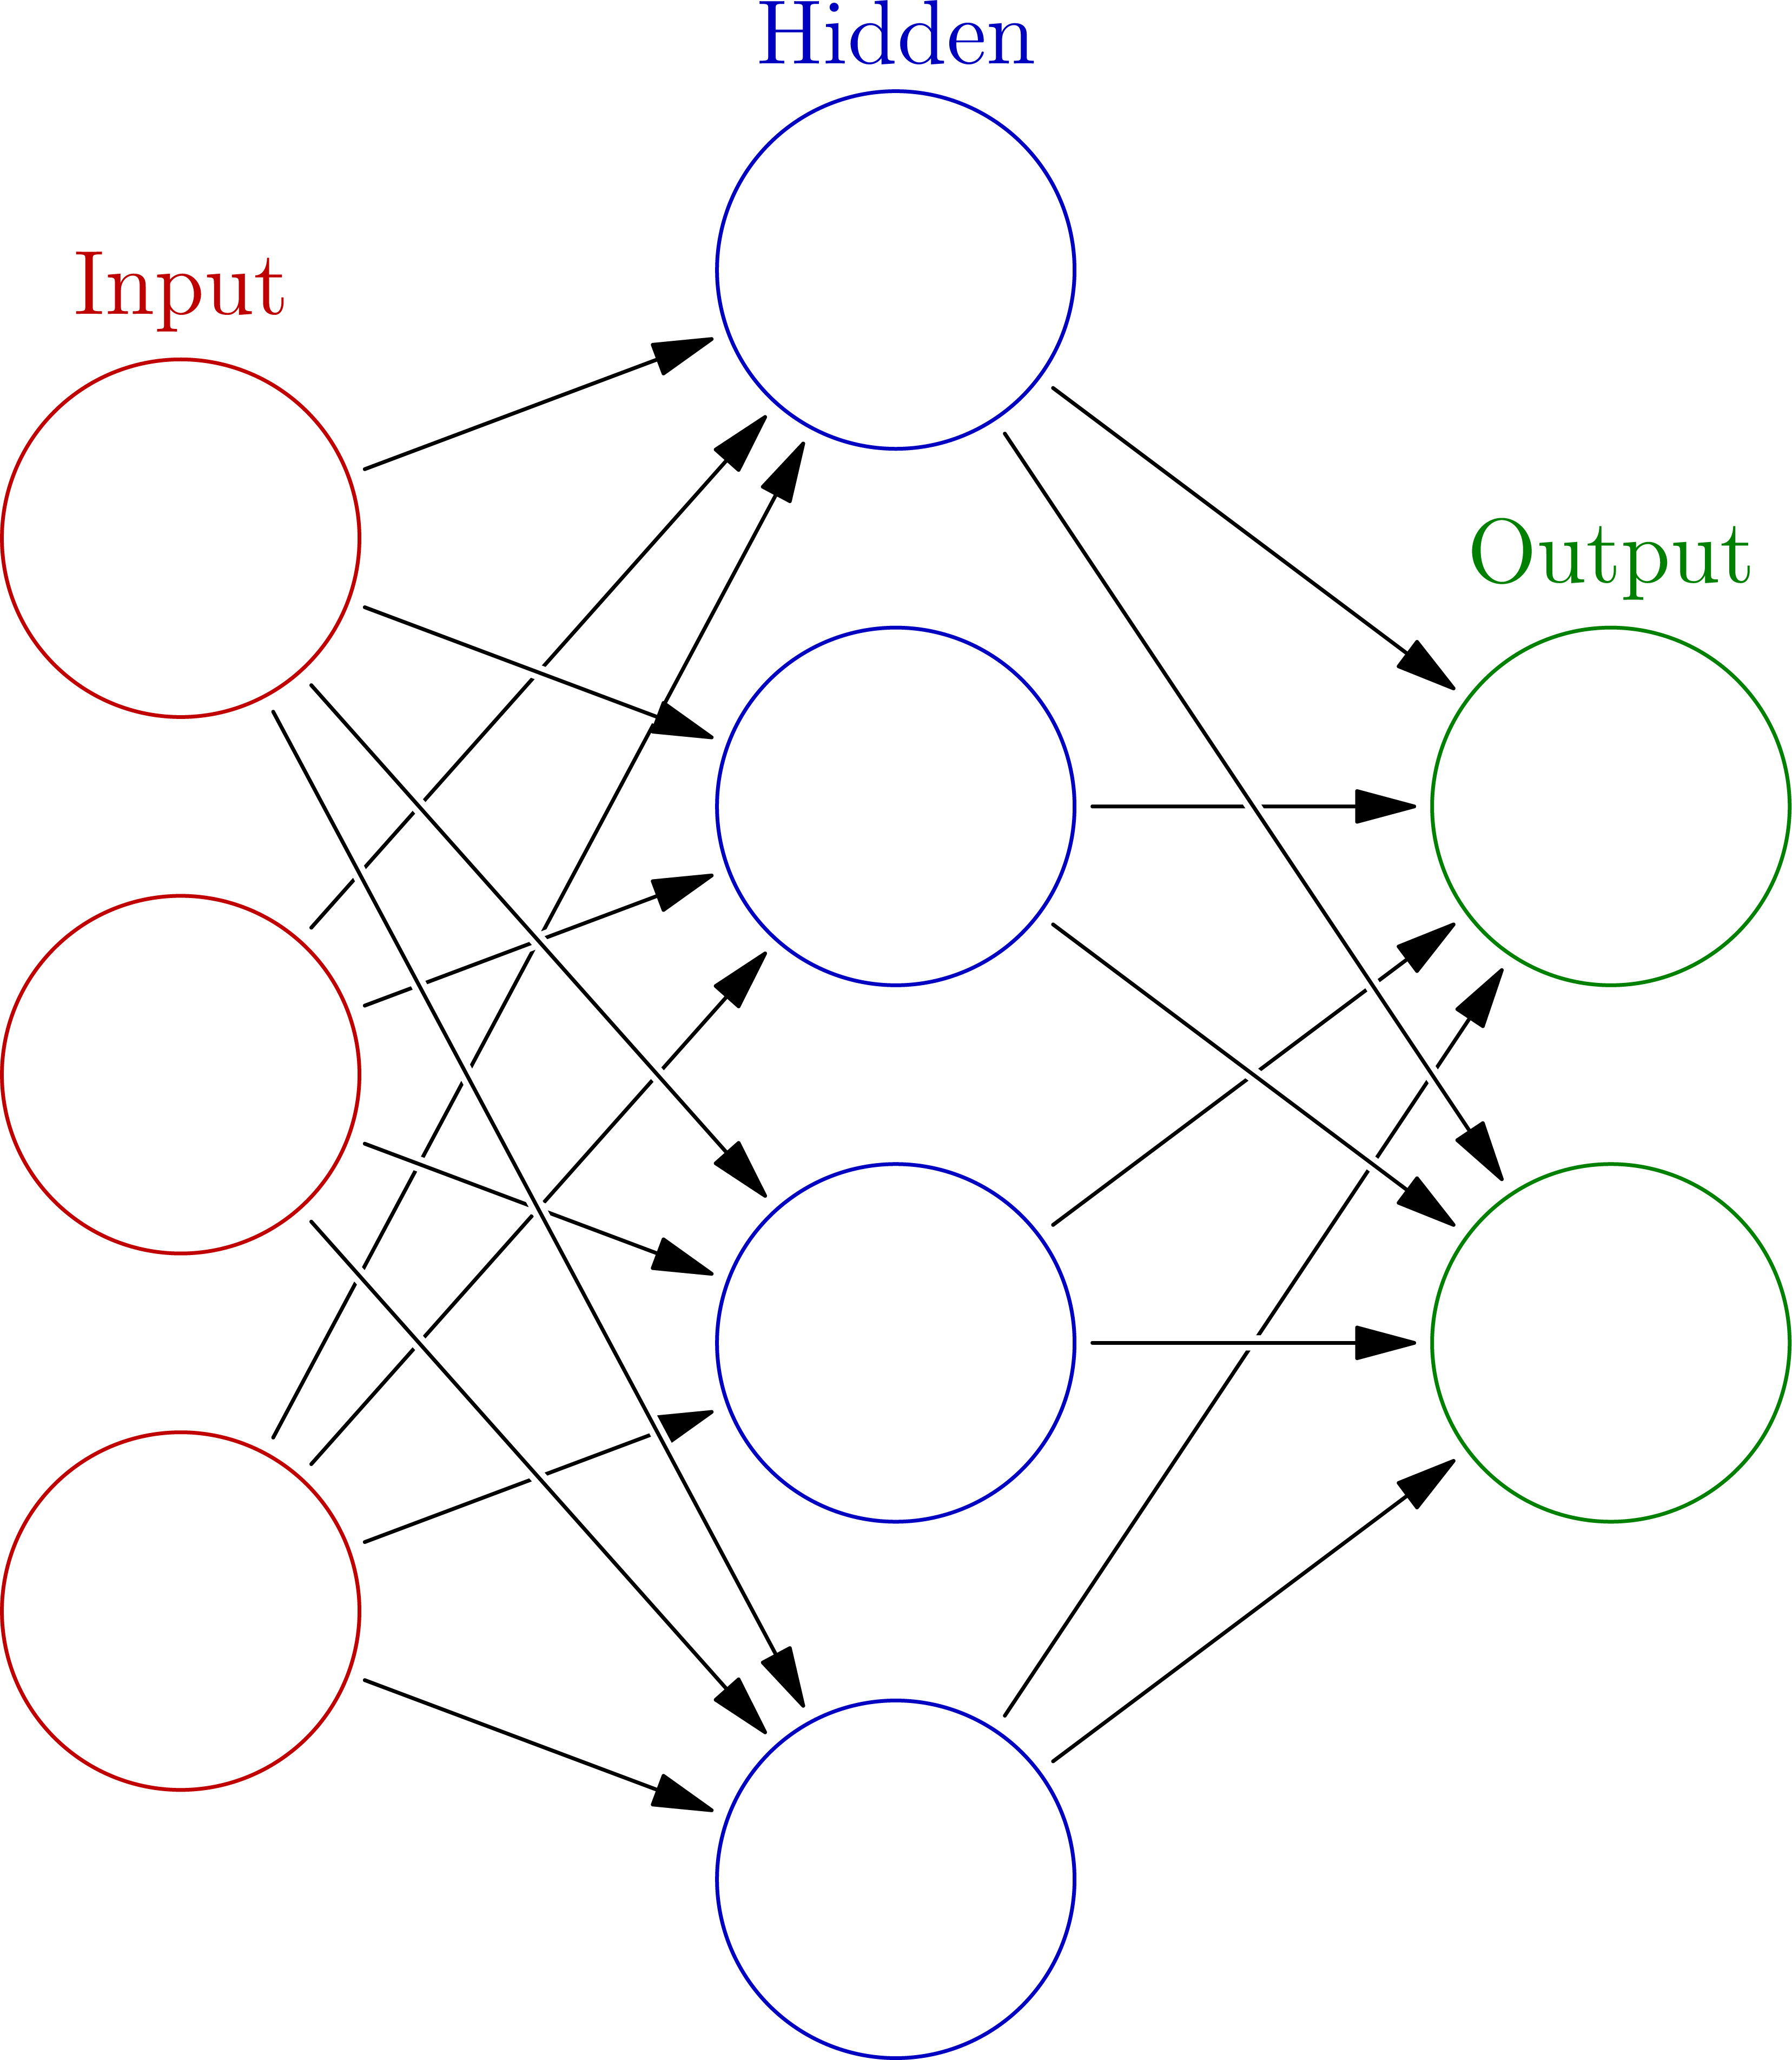
\includegraphics[scale=0.25]{neural_network.png}
\caption{Primer nevronske mreže. vir:
	\href{https://en.wikipedia.org/wiki/Artificial\_neural\_network\#/media/File:Colored\_neural\_network.svg}{Wikipedia}}
\label{slika1}
\end{center}
\end{figure}
\emph{Nevronska mreža} je omrežje povezanih nevronov ali vozlišč.\cite{ann_def_1}
Njena oblika se zgleduje po strukturi živalskih možganov.\cite{ann_def_2}
Podobno se tudi ``uči'': Za vsak učni primer se prilagodi glede na razliko med njenim in ciljnim izhodom.

Prednost nevronske mreže v primerjavi s standardnimi algoritmi je, da za gradnjo mreže postopka iskanja rešitve ni potrebno točno definirati.
Na razpolago moramo imeti le dovolj velik nabor parov vhodnih podatkov in pripadajočih izhodov - \emph{učno množico} - ter dovolj računske moči.
Posledično lahko z njimi rešujemo probleme, ki so preveč kompleksni za direktno algoritmično reševanje ali ko algoritma sploh ne moremo definirati,
	na primer klasifikacija slik, aproksimacija težko izračunljivih funkcij, regresijska analiza \ldots

Slabost nevronske mreže je njena nenatančnost.
Večina nevronskih mrež ne doseže 100\% natančnosti, kar pomeni, da niso primerne za življenjsko kritične namene.
Poleg tega za doseganje dobrih rezultatov zahtevajo ogromne, raznolike učne množice in veliko računskega časa.\cite{ann_compute}

\subsection{Konvolucijska nevronska mreža}

\emph{Konvolucijske nevronske mreže} so eden izmed tipov usmerjenih nevronskih mrež.
Navadno so sestavljene iz več slojev, kjer so posamezni sloji konvolucije, aktivacijske funkcije, združevalne funkcije ali
	\emph{polno povezani sloji} - sloji, pri katerih je vsak nevron vhoda uteženo povezan z vsakim nevronom izhoda.
Združevalne funkcije, kot so max$(A)$, min$(A)$ in avg$(A)$ zmanjšajo količino vmesnih podatkov, kar poenostavi proces učenja.\cite{cnn_pool}

Konvolucije emulirajo odziv nevronov na lastnosti vhodnih stimulusov, podobno kot ljudje bel krog na temnem ozadju zaznamo kot
	vir svetlobe.\cite{cnn_conv}

Pravilno načrtovane konvolucijske nevronske mreže potrebujejo relativno malo preprocesnega dela, kar omogoča hiter in enostaven razvoj programov,
	ki jih uporabljajo.

% 3
\section{Oblika}

\subsection{Načrt mreže}

Mreža je sestavljena iz dveh slojev, in sicer ene konvolucije z jedrom velikosti $k$ ter aktivacijske funkcije pritrditve (ang. \emph{clamp}),
	definirane kot:
\begin{equation*} 
clamp(x) = \begin{cases}
	255 & \text{za } x > 255 \\
	x & \text{za } x \in [0, 255] \\
	0 & \text{za } x < 0
\end{cases}.
\end{equation*}
Tu nelinearnost aktivacijske funkcije ne igra posebne vloge, pomaga pa omejiti izhodno vrednost v dopustno območje števil, ki jih lahko zaokrožimo v
	8-bitno celo število.

Za vhod vzame povečano sliko dimenzij $(\text{širina}, \text{višina})$, vrne pa sliko dimenzij $(\text{širina} - k + 1,\\ \text{višina} - k + 1)$.

Izguba se računa s funkcijo \emph{zglajene linearne izgube}, definirane kot:
\begin{equation*} 
\text{izguba}(\text{izhod}, \text{cilj}) = \frac{1}{n} \sum_{i = 1}^{n} smooth(\text{cilj}_i - \text{izhod}_i),
\end{equation*}
kjer je funkcija $smooth$ definirana kot:
\begin{equation*} 
smooth(x) = \begin{cases}
	0.5 x^2 & \text{za } |x| < 1 \\
	|x| - 0.5 & \text{sicer}.
\end{cases}
\end{equation*}
Ta funkcija ni toliko občutljiva na ekstremne primere kot MSE, ne potrebuje toliko računskega časa kot RMSE in da boljše rezultate kot vsota razdalj,
	ko se mreža približuje optimumu.\cite{smooth_l1}

Za optimizacijo se uporablja algoritem Adam.
Ta je zelo podoben gradientnemu spustu, le da z uporabo dodatnih parametrov pohitri konvergenco k optimumu.\cite{adam}

Vse računanje poteka v številih s plavajočo vejico v enojni natančnosti, \texttt{float32}.

\subsection{Oblika podatkov}

\begin{figure}[htbp]
\begin{center}
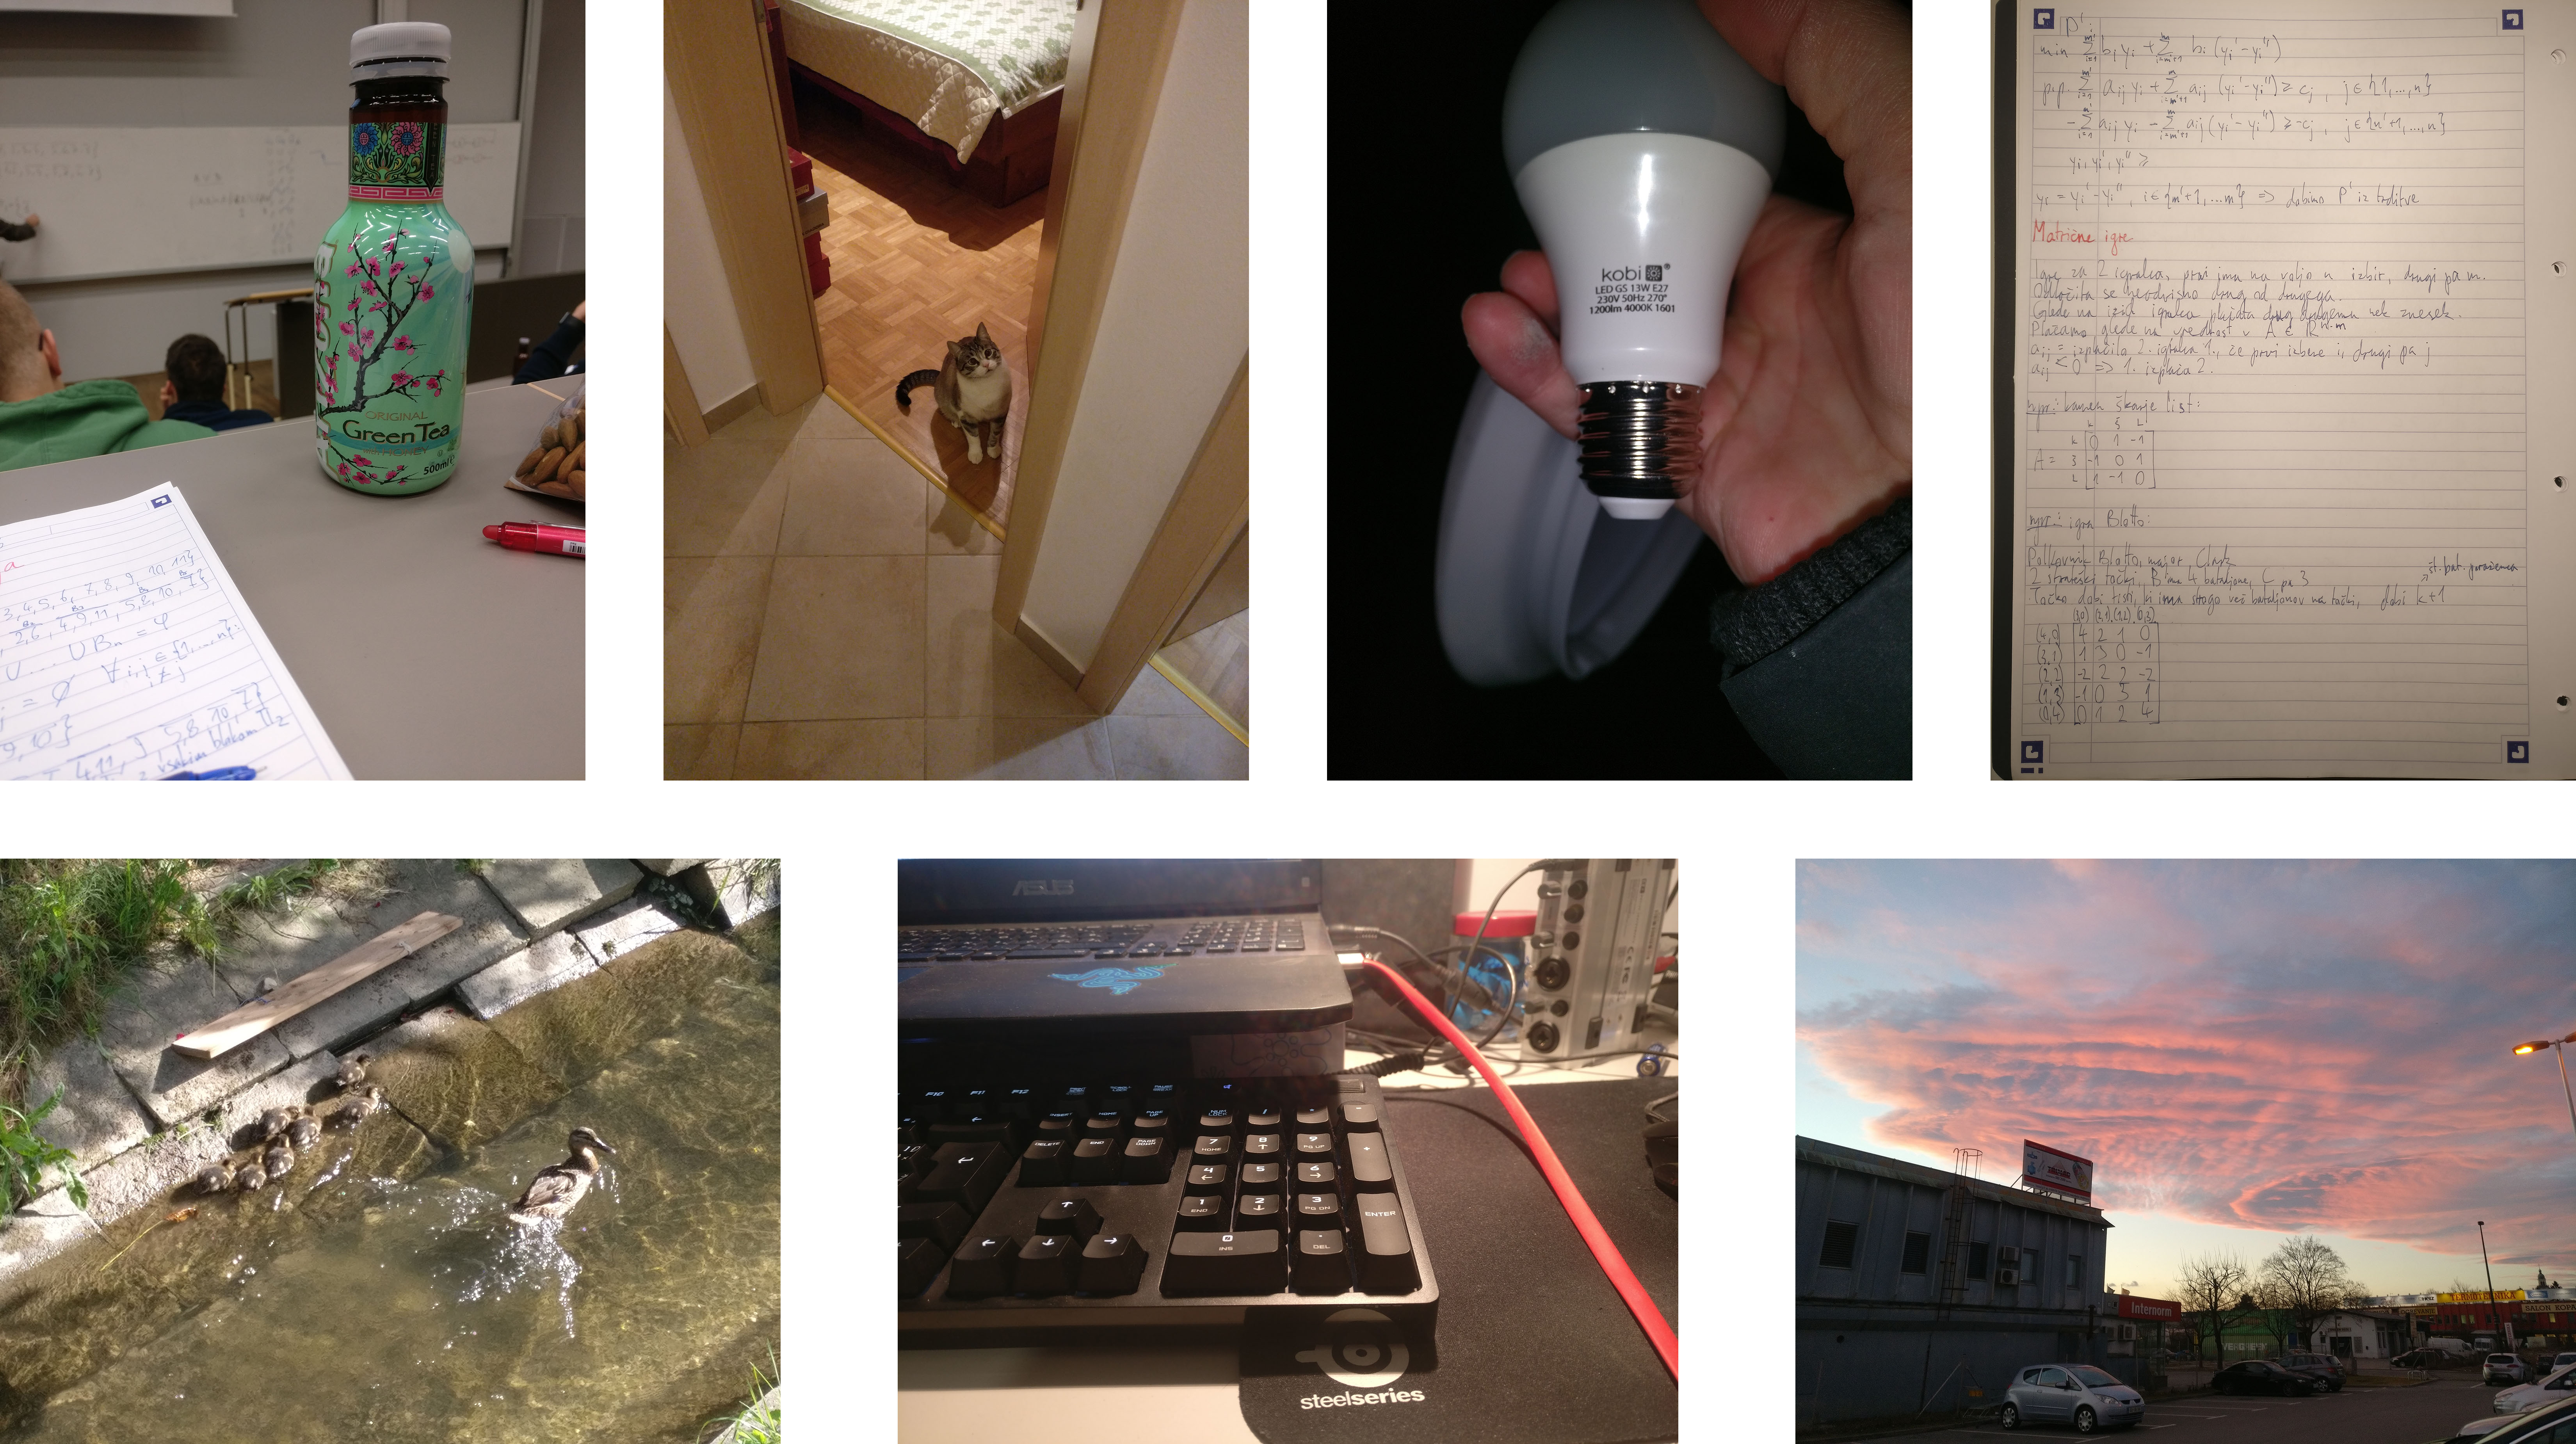
\includegraphics[scale=0.285]{picture_samples.jpg}
\caption{Primeri slik iz množice vhodnih podatkov.}
\label{slika1}
\end{center}
\end{figure}

Za množico vhodnih podatkov sem izbral 644 slik, ki sem jih naredil z mojim pametnim telefonom v obdobju zadnjih dveh let in nekaj mesecev.
Predstavljajo raznolik nabor, slikal sem ljudi, živali, naravo, zapiske, naključne predmete in še kaj.

Velikosti slik so različne, ampak večina jih je oblike (3480, 4640) ali (4640, 3480), kar predstavlja 16M pikslov.
Stisnjene so z le rahlimi izgubami, vsebujejo pa zmerno količino statičnega šuma, kar sem pred učenjem poskušal omiliti z rahlim Gaussovim filtrom.

Slike so razdeljene na dva dela.
Prvi del je učna množica 580 slik, drugi pa testna množica 64 slik.
Slike so bile razdeljene naključno, s funkcijo \texttt{random.sample} v programskem jeziku Python 3.

\section{Programsko okolje}

Mrežo sem implementiral v programskem jeziku Python 3, uporabil sem knjižnico za strojno učenje \href{https://pytorch.org/}{PyTorch}.
Ker sem hotel izvajati učenje na grafični kartici, sem namestil tudi gonilnike za platformo CUDA in knjižnico cuDNN.
Za delo s tenzorji sem uporabil knjižnico \texttt{numpy}, za delo s slikami pa knjižnico \texttt{scikit\_image}.

Vsa izvorna koda je dosegljiva na javnem repozitoriju na naslovu \url{https://github.com/hackguy25/ImgResize}.
Tam so zapisane tudi specifične verzije knjižnic in okolja.

\section{Učenje}

Mrežo sem učil s pomočjo skripte \texttt{train.py}.
Vsako sliko sem naložil z diska, skrčil s faktorjem 4, povečal s faktorjem 4 z bilinearno interpolacijo in jo skupaj z originalom podal mreži.
Ta je na grafični kartici izvedla učni korak z učno hitrostjo $lr$ in vrnila napako pri trenutni sliki.
To napako sem izpisal na standardnem izhodu za lažje sledenje napredku.

Učenje sem izvajal v iteracijah.
V vsaki iteraciji sem na mreži izvedel en korak z vsako izmed 580 slik iz učne množice.
Po vsaki iteraciji sem zmanjšal hitrost učenja, $lr$, tako da so posamezne slike le minimalno pripomogle k neželenemu odstopanju.

Vse učenje sem izvajal na mojem osebnem računalniku s procesorjem AMD Ryzen Thread\-rip\-per
	1920X,\footnote{\url{https://www.amd.com/en/products/cpu/amd-ryzen-threadripper-1920x}}
	32GB pomnilnika in grafično kartico Nvidia 1080 Ti.\footnote{\url{https://www.nvidia.com/en-gb/geforce/products/10series/geforce-gtx-1080-ti/}}

Ker je pretvorba slik potrošila veliko več časa kot samo učenje, sem postopek paraleliziral s pomočjo Pythonovega modula \texttt{multiprocessing}.
V vsakem koraku sem naenkrat pretvoril 12 slik, vsako v svojem procesu, in izvedel učenje na 12 slikah iz prejšnjega koraka.
Tako sem dosegel do 90\% povprečno izkoriščenost procesorja in 60\% povprečno izkoriščenost grafične kartice tekom postopka učenja.

Ustvaril sem dve različici mreže, ki se razlikujeta le v jedru konvolucije in času učenja.

Prva različica ima jedro velikosti $17 * 17$, učenje pa je potekalo v 15 iteracijah, kjer je bila hitrost učenja v $i$-ti iteraciji podana tako:
\begin{equation*} 
lr = 0.00001 \cdot 0,33^{i - 1}
\end{equation*}

Druga različica ima jedro velikosti $25 * 25$, učenje pa je potekalo v 30 iteracijah, kjer je bila hitrost učenja v $i$-ti iteraciji podana tako:
\begin{equation*} 
lr = 0.00001 \cdot 0,85^{i - 1}
\end{equation*}

Kljub večjemu jedru konvolucije druge različice učenje ni potekalo občutno počasneje.

Pri obeh različicah sem za izvedbo ene iteracije potreboval povprečno 12 minut.
Za učenje prve različice sem porabil približno 3 ure, za učenje druge pa približno 6.
Povprečna poraba energije računalnika med učenjem je nihala med 400 in 450W, torej sem za učenje obeh različic porabil nekje med 3,5 in 4 kWh električne
	energije.

\section{Testiranje}

Obe različici mreže sem testiral na 64 slikah iz testne množice.
Slike sem predhodno skrčil na četrtino velikosti v vsako dimenzijo, nato pa jih obdelal z obema različicama mreže.
Slika 3 prikazuje nekaj primerov povečanih slik, v primerjavi z bilinearno in bikubično interpolacijo.

\begin{figure}[htbp]
\begin{center}
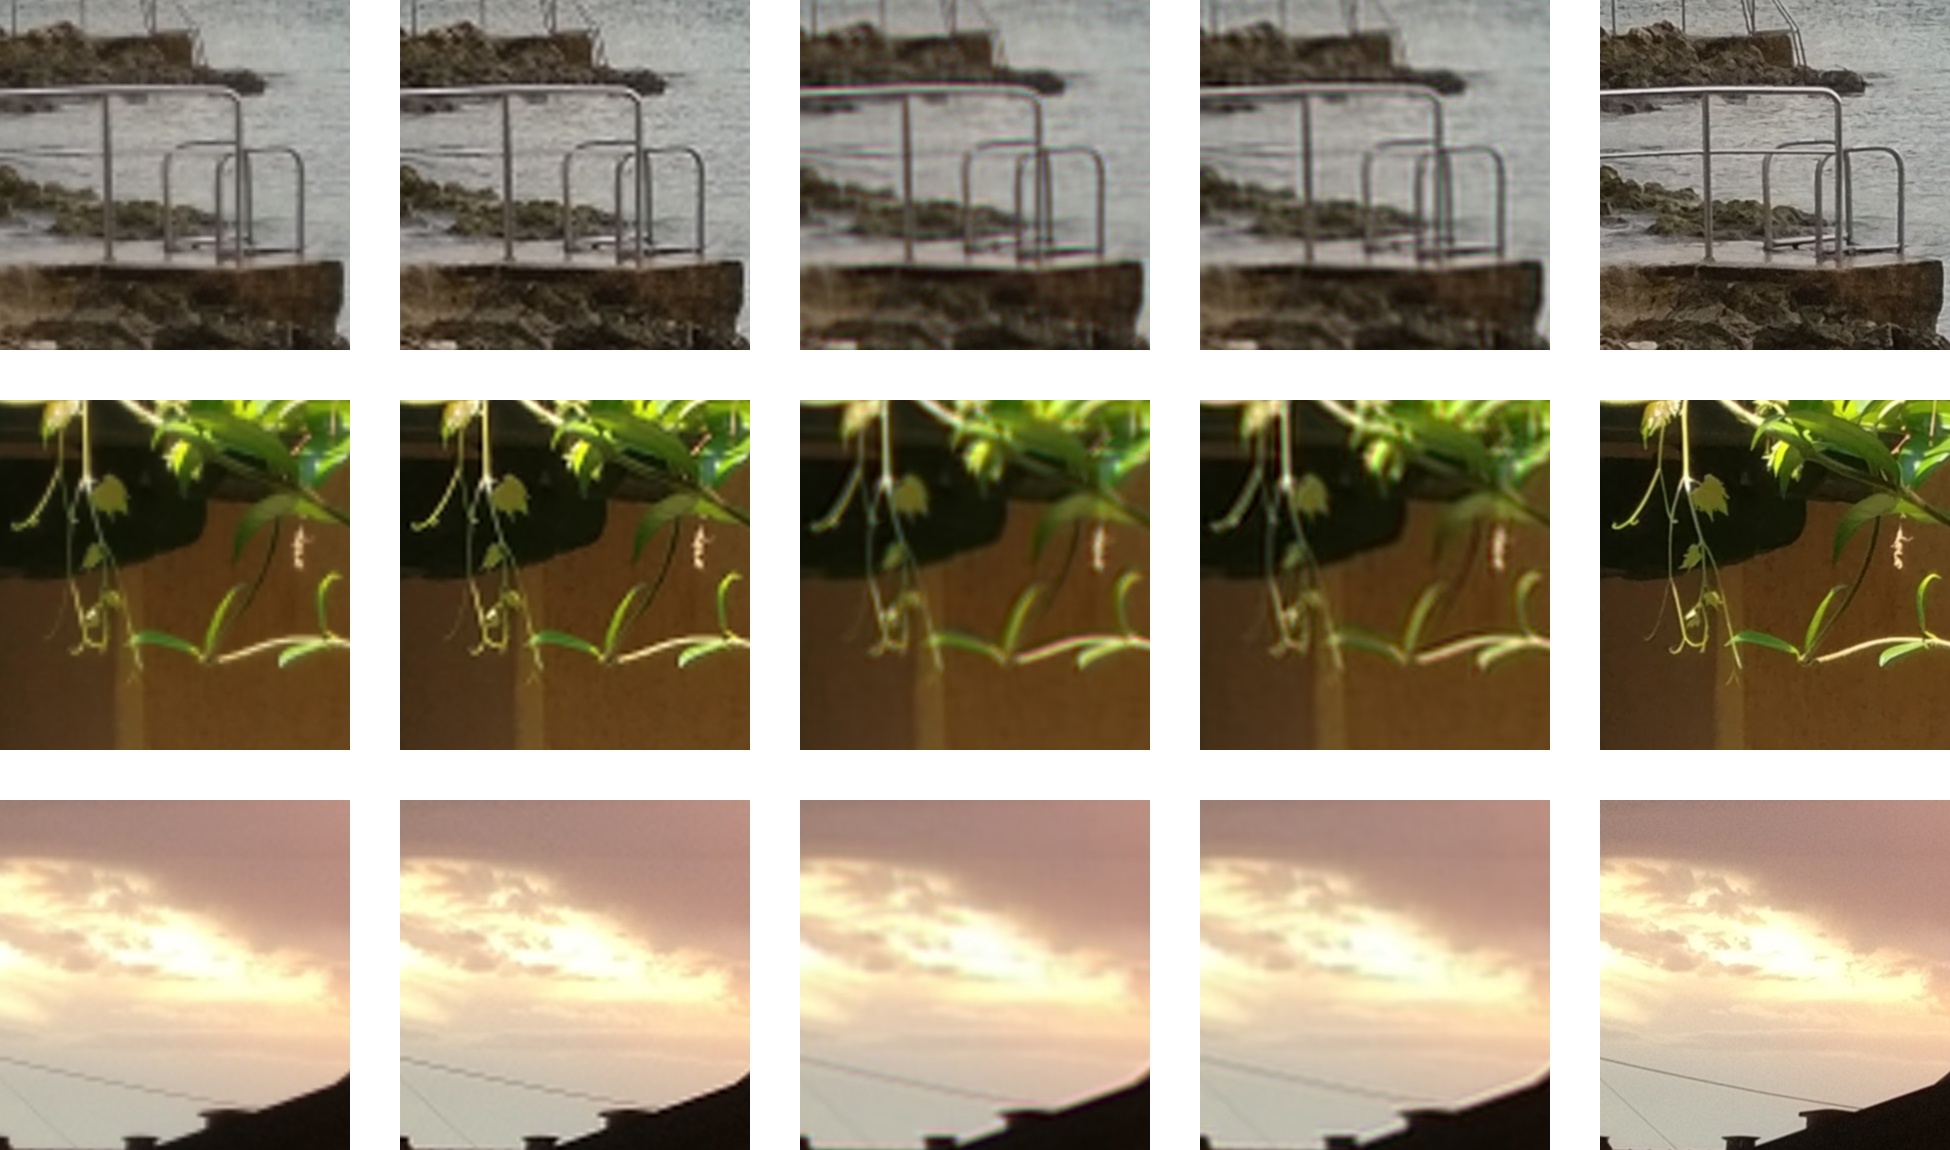
\includegraphics[scale=0.231]{picture_comparison.jpg}
\caption{Primeri slik iz množice vhodnih podatkov, z leve: bilinearno, bikubično, konvolucija $17 * 17$, konvolucija $25 * 25$, izvorna slika}
\label{slika1}
\end{center}
\end{figure}

\section{Zaključek}

Povečava slik z mrežo se od povečave z eno izmed obstoječih interpolacij najbolj razlikuje večinoma v tem, da mreža ne ohranja toliko ostrine kot 
	interpolacija, ampak veliko bolje ohranja obliko ostrih prehodov svetlosti.

Najbolj pozitivno bi na kvaliteto izhodnih slik vplivala večja učna množica, 580 slik ni veliko v primerjavi s prosto dostopnimi nabori
	slik.\cite{datasets}
Lahko bi tudi povečal število učnih iteracij, ampak že pri zadnjih iteracijah obstoječega učnega postopka so bile razlike minimalne.
Uporabil bi lahko tudi večja jedra konvolucije, ampak glede na relativno majhno razliko med različicama menim, da pridobitek ne bi upravičil dodatne
	kompleksnosti.

Kljub tem pomanjkljivostim mislim, da je bila izdelava mreže uspeh.

\begin{thebibliography}{99}

% članek na spletni strani: \bibitem{tag} Avtor. (leto). Naslov. \emph{Stran/publikacija}. [Online] Dosegljivo: \url{url}. [Dostopano \today].
% študija: \bibitem{tag} Avtor, ``Naslov''. Institucija, (št.poročila, datum).

\bibitem{intel1} Alberto V\@. (2017). An Example of a Convolutional Neural Network for Image Super-Resolution.
	\emph{Intel AI Academy} [Online]. Dosegljivo:
	\url{https://software.intel.com/en-us/articles/an-example-of-a-convolutional-neural-network-for-image-super-resolution}.
	[Dostopano \today].

\bibitem{intel2} Chao Dong \emph{et al}., ``Learning a Deep Convolutional Network for Image Super-Resolution''. The Chinese University of Hong Kong.

\bibitem{intel3} Jiwon Kim \emph{et al}., ``Accurate Image Super-Resolution Using Very Deep Convolutional Networks''.
	Seoul National University, Korea.

\bibitem{torch_conv2d} \texttt{torch.nn.Conv2d}. \url{https://pytorch.org/docs/stable/nn.html}. [Dostopano \today].

\bibitem{activation_func_1} ``What is an Activation Function?''. \url{https://deepai.org/machine-learning-glossary-and-terms/activation-function}.
	[Dostopano \today].

\bibitem{activation_func_2} Avinash Sharma V\@. (2017). Understanding Activation Functions in Neural Networks. \emph{The Theory Of Everything}.
	[Online] Dosegljivo: \url{https://medium.com/the-theory-of-everything/understanding-activation-functions-in-neural-networks-9491262884e0}.
	[Dostopano \today].

\bibitem{ann_def_1} J.~ J.~ Hopfield. (1982). Neural networks and physical systems with emergent collective computational abilities.
	\emph{Proceedings of the National Academy of Sciences of the United States of America}. [Online] Dosegljivo:
	\url{http://www.pnas.org/content/pnas/79/8/2554.full.pdf}. [Dostopano \today].

\bibitem{ann_def_2} Marcel van Gerven, Sander Bohte. (2018). Artificial Neural Networks as Models of Neural Information Processing.
	\emph{Frontiers in Computational Neuroscience}. [Online] Dosegljivo:
	\url{https://www.frontiersin.org/research-topics/4817/artificial-neural-networks-as-models-of-neural-information-processing}.
	[Dostopano \today].

\bibitem{ann_compute} Chris Edwards. (2015). \emph{Growing pains for deep learning}. Communications of the ACM. 58 (7): 14–16.

\bibitem{cnn_conv} \emph{Convolutional Neural Networks (LeNet) – DeepLearning 0.1 documentation}. DeepLearning 0.1. LISA Lab.
	[Online] Dosegljivo: \url{http://deeplearning.net/tutorial/lenet.html}. [Dostopano \today].

\bibitem{cnn_pool} Alex Krizhevsky \emph{et al}. (2012). ImageNet Classification with Deep Convolutional Neural Networks.
	\emph{NIPS 2012}. [Online] Dosegljivo: \url{http://www.image-net.org/challenges/LSVRC/2012/supervision.pdf}. [Dostopano \today].

\bibitem{smooth_l1} Ross Girshick. (2015). Fast R-CNN. \emph{Microsoft Research}. [Online] Dosegljivo: \url{https://arxiv.org/pdf/1504.08083.pdf}.
	[Dostopano \today].

\bibitem{adam} Diederik P. Kingma, Jimmy Lei Ba. (2015). Adam: A Method for Stochastic Optimization.
	\emph{International Conference for Learning Representations}. [Online] Dosegljivo: \url{https://arxiv.org/pdf/1412.6980.pdf}. [Dostopano \today].

\bibitem{datasets} \emph{Datasets}. Deep Learning. [Online] Dosegljivo: \url{http://deeplearning.net/datasets/}. [Dostopano \today].

\end{thebibliography}

\end{document}
